% !TeX document-id = {54177b55-cdde-488b-90fe-107922d59049}
\documentclass[12pt]{article}

\usepackage{a4} 
\usepackage{amsmath}
\usepackage{amssymb}
\usepackage[]{xcolor}
\usepackage{graphicx}
\usepackage[colorlinks,urlcolor=blue,linkcolor=blue,citecolor=hotpink]{hyperref}
\usepackage{booktabs}
\usepackage{rotating}
\usepackage{caption}
\usepackage[british]{babel}
\usepackage[linesnumbered, ruled]{algorithm2e}
\usepackage{epstopdf}
\usepackage{mathtools} % for :=
\usepackage{subfig}
\usepackage[most, minted]{tcolorbox}
\usepackage{mdwlist}
\tcbuselibrary{listings}
%\usepackage[cache=false]{minted} % Need cache=false or leads to funny bug.
% !TeX TXS-program:compile = txs:///pdflatex/[--shell-escape]

\newtcblisting{myminted}{%
	listing engine=minted,
	minted language=python,
	listing only,
	breakable,
	enhanced,
	minted options = {
		linenos, 
		breaklines=true, 
		breakanywhere, 
		fontsize=\footnotesize, 
		numbersep=2mm,
		tabsize=2
	},
	overlay={%
		\begin{tcbclipinterior}
			\fill[gray!25] (frame.south west) rectangle ([xshift=4mm]frame.north west);
		\end{tcbclipinterior}
	}   
}
\BeforeBeginEnvironment{minted}{\begin{tcolorbox}[breakable, enhanced]}%
	\AfterEndEnvironment{minted}{\end{tcolorbox}}%


\graphicspath{{images/}}

\title{Critical path estimation in heterogeneous scheduling heuristics} % Think of a better title...
\author{Thomas McSweeney%
	\thanks{%
		School of Mathematics,
		University of Manchester,
		Manchester, M13 9PL, England
		(\texttt{thomas.mcsweeney@postgrad.manchester.ac.uk}).
	}
}
\date{\today}

%%%%%%%%%%%%%%%%%%%%%%%%%%%%%%%%%
\def\R{\mathbb{R}}
\def\C{\mathbb{C}}
\def\P{\mathbb{P}}
\def\E{\mathbb{E}}
\def\nbyn{n \times n}
\def\mbyn{m \times n}
\def\l{\lambda}
\def\norm#1{\|#1\|}      
\def\normi#1{\|#1\|_1}
\def\normo#1{\|#1\|_{\infty}}
\def\Chat{\widehat{C}}
\def\e{eigenvalue}
\DeclareMathOperator*{\argmax}{arg\,max}
\DeclareMathOperator*{\argmin}{arg\,min}

% \DeclareMathOperator{\diag}{diag}   % Requires amsmath.
\def\diag{\mathop{\mathrm{diag}}}     % If not using amsmath.
\def\trace{\mathop{\mathrm{trace}}}   % If not using amsmath.

\def\At{\widetilde{A}}
\def\normt#1{\|#1\|_2}

% Set up lemma environment and its numbering.
\newtheorem{lemma}{Lemma}[section]

\def\proof{\par{\bf Proof}. \ignorespaces}
\def\qedsymbol{\vbox{\hrule\hbox{%
			\vrule height1.3ex\hskip0.8ex\vrule}\hrule}}
\def\endproof{\qquad\qedsymbol\medskip\par}

\newtheorem{theorem}{Theorem}
\newtheorem{prop}[theorem]{Proposition}

\allowdisplaybreaks[1]

%%%%%%%%%%%%%%%%%%%%%%%%%%%%%%%%%%%%%%%%%%%%%%%%%%%%%%%%%%%%%%%%%%%%%%%%%%%%
% For fine-tuning spacing in \sqrt etc=.  From \cite[p.~155]{knut99}.
% In math mode, @ will act as a macro that adds 1 unit of space.
% By comparison, \, skips 3mu.

\mathcode`@="8000 % Make @ behave as per catcode 13 (active).  TeXbook p. 155.
{\catcode`\@=\active\gdef@{\mkern1mu}}
%%%%%%%%%%%%%%%%%%%%%%%%%%%%%%%%%%%%%%%%%%%%%%%%

%%%%%%%%%%%%%%%%%%%%%%%%%%%%%%%%%%%%%%%%%%%%%%%%%%%%%%%%%%%%%%%%%%%%%%%%%%%%
\newcounter{mylineno}
\makeatletter
\let\oldtabcr\@tabcr
\def\nonumberbreak{\oldtabcr\hspace{3.5pt}}
\def\mynewline{\refstepcounter{mylineno}%
	\llap{\footnotesize\arabic{mylineno}\hspace{5pt}}%
}
\def\lineref#1{\footnotesize\ref{#1}}
% Next macro adapted from latex.ltx
\gdef\@tabcr{\@stopline \@ifstar{\penalty%
		\@M \@xtabcr}\@xtabcr\mynewline}
\def\myvspace#1{\oldtabcr[#1]\mynewline}
\newenvironment{code}{%
	% Swap `:' and `colon'...
	\mathcode`\:="603A  % TeXbook pp 134, 154, 359 (top)
	% For original colon     \mathcode`\:="303A  % TeXbook p 344
	\def\colon{\mathchar"303A}
	\setcounter{mylineno}{0}
	\par
	\upshape
	\begin{list} % To give indentation
		{} {\leftmargin = 1cm}
		\item[]
		\begin{tabbing}
			
			% Default tab stops
			\hspace*{.3in} \= \hspace*{.3in} \=
			\hspace*{.3in} \= \hspace*{.3in} \= \kill
			\mynewline
		}{\end{tabbing}\end{list}}
\makeatother


\addto\captionsbritish{	\renewcommand{\bibname}%
	{References}%TODO: make sure reference style is consistent.
}

\definecolor{hotpink}{rgb}{0.9,0,0.5}

\begin{document}
	\maketitle 	


\section{Introduction}
\label{sect.intro}

%Before describing HEFT, we first introduce the concept of the {\em critical path}. The name comes from project management, where it is defined as the longest sequence of activities that must be done in order to complete a project \cite{kel59,kel61}; for a task graph, the critical path is the longest (costliest) path through it. This is useful because, if we assume sufficient parallelism, then the time it takes to execute the tasks on the critical path of a DAG therefore gives a lower bound on the makespan of any schedule. A natural approach in a listing heuristic then is to prioritize all tasks according to the length of the critical path from that task to the end; the idea being that tasks with the greatest downward path length contribute most towards the makespan and should therefore be processed as soon as possible. This approach has a long and successful history in scheduling for homogeneous processors \cite{cof72} but it isn't clear how it should be defined for heterogeneous ones, when all DAG costs can take multiple values and there are many possible critical paths (see Chapter \ref{chap.critical_path_estimation}).

Recall from previous chapters that the {\em Heterogeneous Earliest Finish Time} (HEFT) heuristic prioritizes all tasks $t_i$, $i = 1, \dots, n$, by recursively computing a corresponding sequence of numbers $u_i$ which are intended to represent {\em critical path} lengths from each task to the end. As noted previously, however, the concept of the critical path is not clearly defined for heterogeneous target platforms: DAG weights are not fixed at this stage so there are multiple ways we could define a {\em longest} (i.e., costliest) path. Consider for example the simple DAG shown in Figure \ref{plot.simple_example}, where the labels represent all the possible weights each task/edge may take on a two-processor target platform; specifically, the labels $(W_i^1, W_i^2)$ near the nodes represent the computation costs on processors $P1$ and $P2$, respectively, while the edge labels $(0 = W_{ik}^{11} = W_{ik}^{22}, W_{ik}^{12}, W_{ik}^{21})$ represent the possible communication costs. What is the longest path through this graph? 

\begin{figure}
	\centering	
	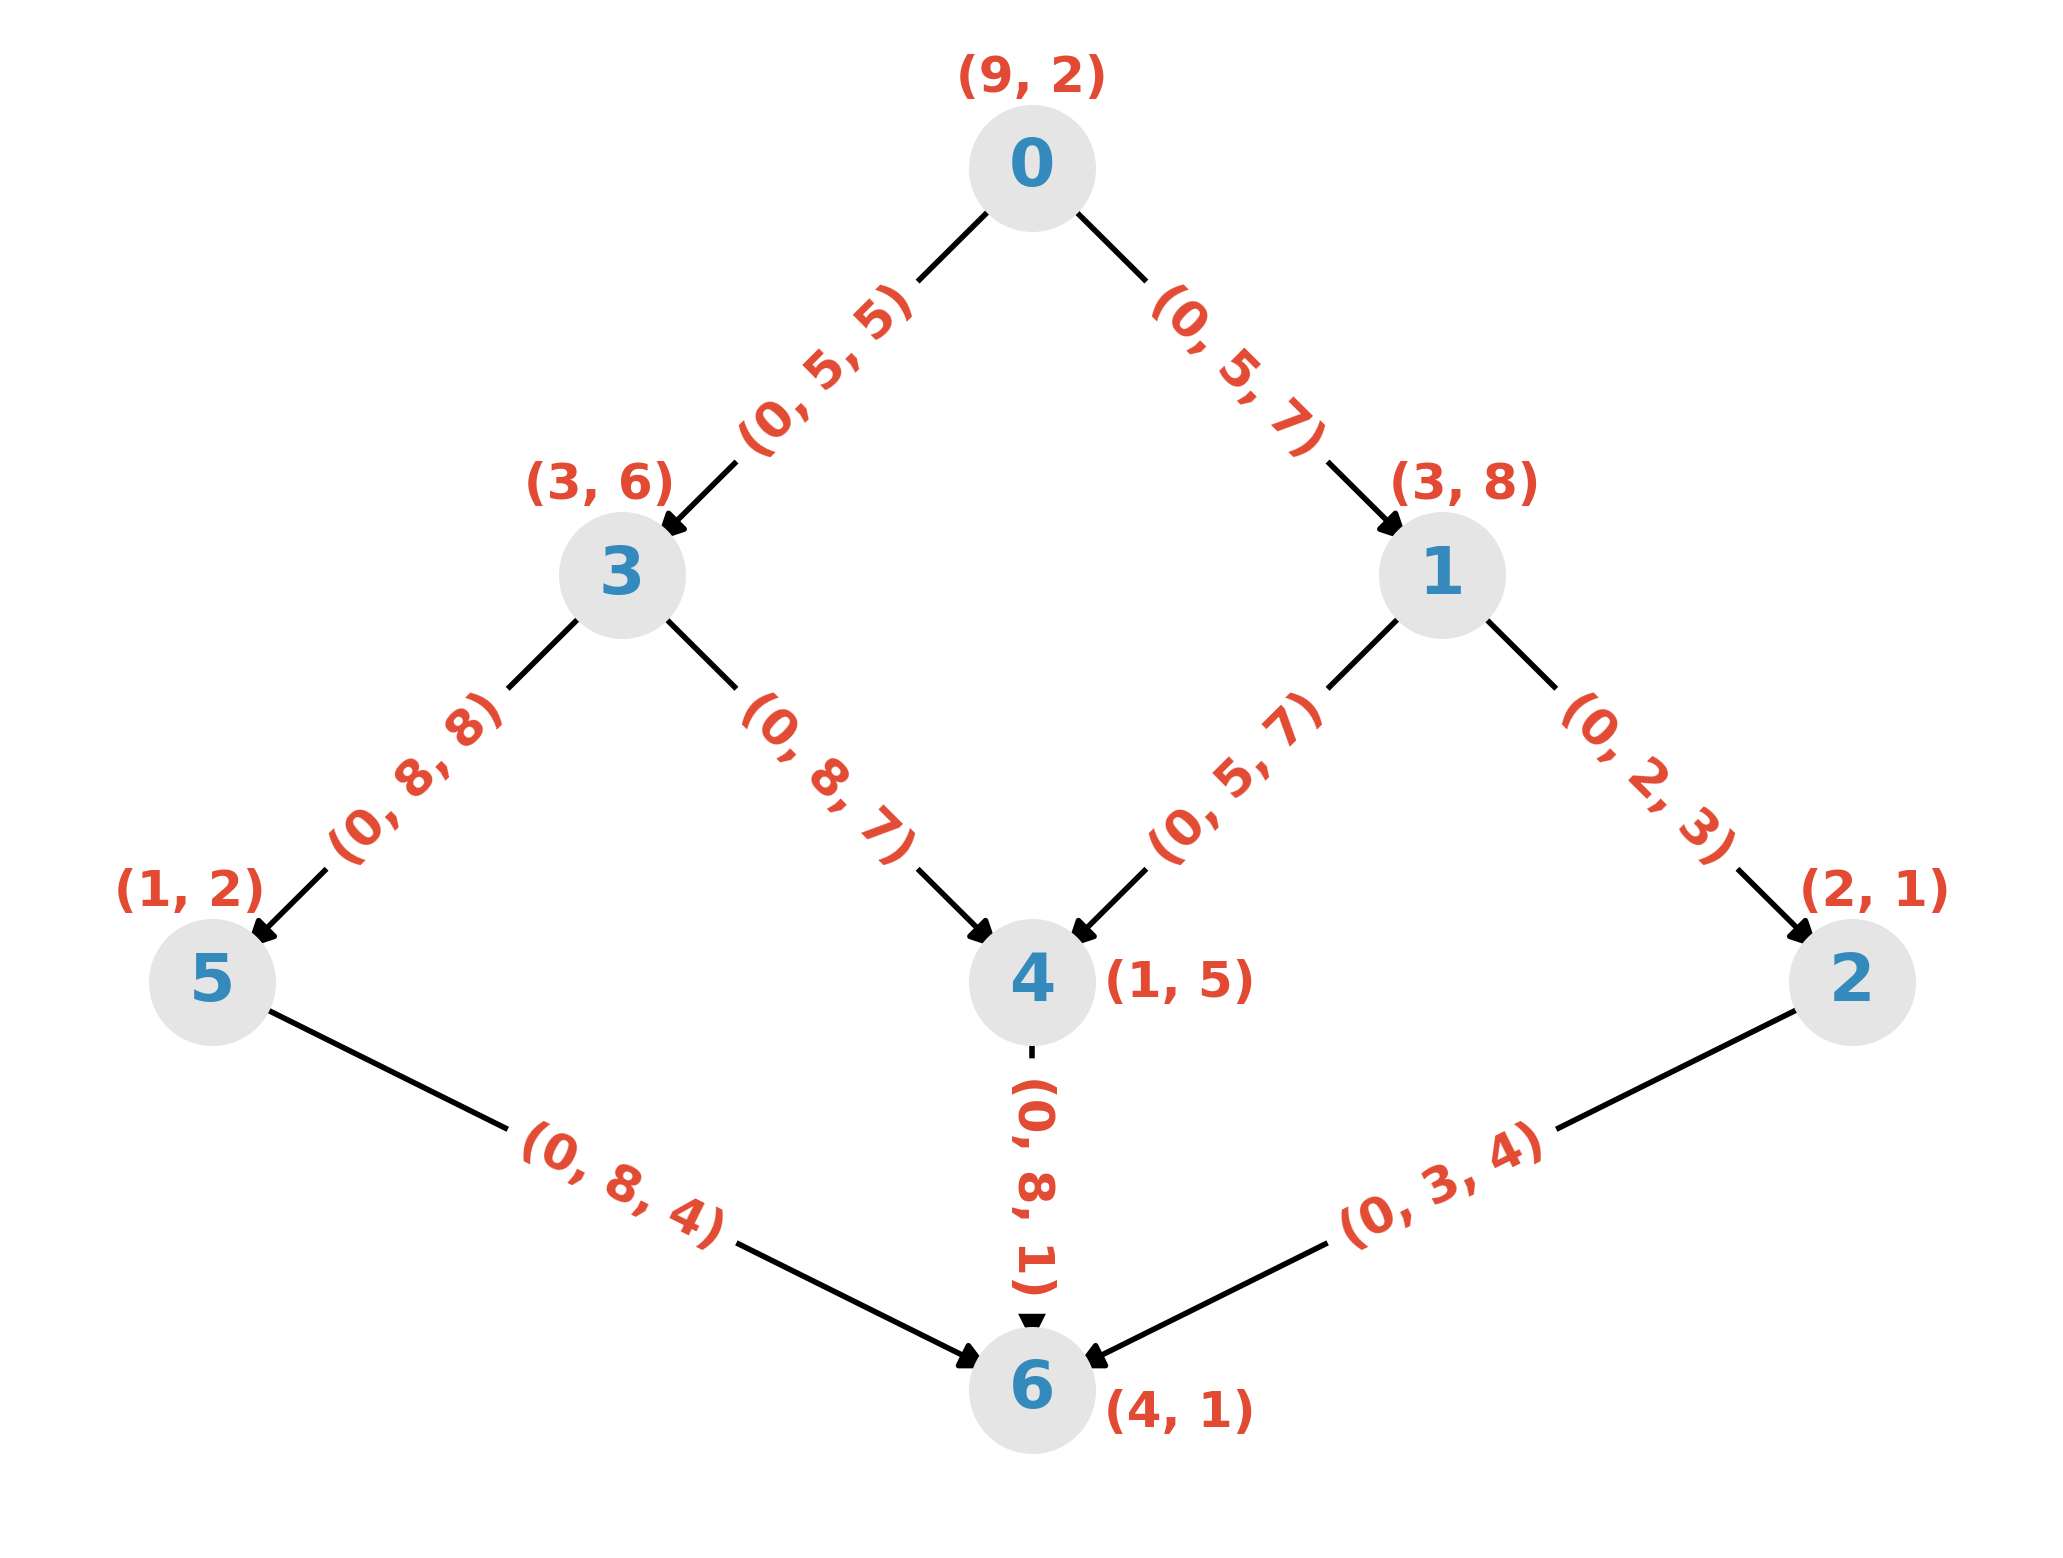
\includegraphics[scale=0.7]{simple_graph.png}
	\caption{Simple task graph with costs on a two-processor target platform.}	
	\label{plot.simple_example}
\end{figure}

It is not obvious how this should be defined. The HEFT approach, as described in previous chapters, is to use mean values over all sets of possible costs to fix the DAG weights and then compute the critical path lengths in a standard dynamic programming manner. For the example, this gives
\begin{align*}
u_6 &= 2.5, \; u_5 = 7, \; u_4 = 7.75, \; u_3 = 16, \\
u_2 &= 5.75, \; u_1 = 16.25, \; \text{and} \; u_0 = 24.75,
\end{align*}
giving a scheduling priority list of $\{0, 1, 3, 4, 5, 2, 6\}$. The schedule length obtained by HEFT with these priorities is 22, so note in particular that $u_0$, the rank of the single entry task, is not a lower bound on this value, unlike in the homogeneous case. The question then is, what quantity do the $u_i$ values actually represent? The most intuitive interpretation is perhaps that the HEFT ranks are estimates of what the critical paths are {\em likely} to be but there is no robust mathematical justification for believing that such a definition is truly the most useful.  

Given this ambiguity, alternative ways to define the critical path in HEFT have been considered before, most notably by Zhao and Sakellariou \cite{zhao03}, who empirically compared the performance of HEFT when averages other than the mean (e.g., median, maximum, minimum) are used to compute upward (or downward) ranks. Their conclusions were that using the mean is not clearly superior to other averages, although none of the other options were consistently better. Indeed, perhaps the biggest takeaway from their investigation was that HEFT is very sensitive to how priorities are computed, with significant variation being seen for different graphs and target platforms. In this chapter we undertake a similar investigation with the aim of establishing if there are choices which do consistently outperform the standard HEFT task ranking phase.   

This will be an empirically-driven study, as is common in this area. To facilitate this investigation we created a software package that simulates heterogeneous scheduling problems, much like that described in the previous chapter, although not restricted to accelerated target platforms. As before, the ({\tt Python}) source code for this simulator can be found on Github\footnote{\href{https://github.com/mcsweeney90/critical-path-estimation}{{\tt \small https://github.com/mcsweeney90/critical-path-estimation}}} and all of the results presented here can be re-run from scripts contained therein. 

% TODO: mention that only giving equations etc for u_i but can analagously define d_i. 

\section{Optimistic bounds}
\label{sect.optimistic}

Functionally, the critical path is used in HEFT as a lower bound on the makespan, so that minimizing the critical path gives us the most scope to minimize the makespan (assuming we make good use of our parallel resources). With this in mind, there are many different ways we can define the critical path so that it gives a lower bound on the makespan of any possible schedule. The most straightforward approach would be to just set all weights to their minimal values but a tighter bound can be computed in the following manner. First, define $O_i^a$ for all tasks $t_i$ and processors $p_a$ to be the critical path length from $t_i$ to the end (inclusive), assuming that it is scheduled on processor $p_a$. These values can easily be computed recursively by setting $O_i^a = W_i^a \; \forall a$ for all exit tasks then moving up the DAG and setting 
\begin{align}
O_i^a &= W_i^a + \max_{k \in S_i} \bigg( \min_{b = 1, \dots, q} \big( O_k^b + W_{ik}^{ab} \big)  \bigg) \quad \forall a \label{eq.opt_uia} 
\end{align}
for all other tasks. Then for each $i = 1, \dots, n$,
\begin{align}
O_i &= \min_{a = 1, \dots, q}O_i^a \label{eq.opt_ui} 
\end{align}
gives a true lower bound on the remaining cost of any schedule once the execution of task $t_i$ begins. These $O_i$ values could be useful as alternative task priorities in HEFT, especially since the cost of computing all of the $O_i^a$ in this manner is only $O(m + n) \approx O(n^2)$ so in particular is no more expensive than the usual HEFT prioritization phase. For example, for the simple graph shown in Figure \ref{plot.simple_example}, we find that the $O_i$ values are as given in Table \ref{tb.opt_example} (with the $u_i$ included for comparison). Interestingly, we see that tasks 1 and 3 have the same optimistic rank (8) and the performance of the alternative ranks relative to the standard $u_i$ sequence in HEFT depends on which is chosen to be scheduled first; if task 1, the priority list does not change so the schedule makespan is 22, but if task 3 is selected instead, the final schedule makespan is 20---smaller than the original.

\begin{table}
	\caption{Upward and optimistic ranks.} 
	\begin{center}	
		\begin{tabular}{c c c}
			\cmidrule{1-3}
			Task & Upward rank & Optimistic rank\\
			\cmidrule{1-3}
			$0$ & $24.75$ & $16$ \\
			$1$ & $16.25$ & 8 \\
			$2$ & $5.75$ & 2 \\
			$3$ & $16$ & 8 \\
			$4$ & $7.75$ & 5 \\
			$5$ & $7$ & 3 \\
			$6$ & $2.5$ & 1 \\
			\bottomrule
		\end{tabular}
		\label{tb.opt_example}
	\end{center}	
\end{table}

Of course, this is only one example: it should be emphasized here that there is absolutely no mathematically valid reason to suppose that using the $O_i$ sequence instead of $u_i$ as the task ranks in HEFT will actually lead to superior performance in general. Still, it seems worthwhile to investigate this empirically using our simulator, which we do in Section \ref{sect.experimental_rankings}. 

%Although taking the minimum over the set of processors as in \eqref{eq.opt_ui} is the only choice that gives a true lower bound, we could use any other average over the set of processors, such as the mean or maximum, in order to compute task priorities. Since we also consider those two alternatives in Section \ref{sect.experimental_rankings}, we refer to the ranking phase defined by using the minimum, maximum and mean as OPT-MIN, OPT-MAX and OPT-MEAN respectively.    

(Note that the optimistic critical path defined here is extremely similar to the optimistic cost used in the PEFT heuristic; this will be discussed further in Section \ref{sect.processor_selection}.)


\section{Stochastic interpretation}
\label{sect.alt_rankings}

In this section we propose a family of alternative task ranking phases in HEFT based on the following interpretation of the standard ranking phase. First, note that by using average values over all sets of possible task and edge costs, HEFT is implicitly assuming that any member of any set is just as likely to be incurred as any other; conceptually, HEFT is attempting to account for the uncertainty of the processor selection phase by assuming that for any given task all processors are equally likely to ultimately be chosen. So, effectively, at the prioritization phase HEFT views the node and edge weights as independent discrete random variables (RVs) with associated probability mass functions (pmfs) given by the aforementioned assumption. More precisely, let $m_i$ be the pmf corresponding to the task weight variable $w_i$ and $m_{ik}$ that for the edge weight $w_{ik}$, then  
\begin{align*}
m_i(W_i^a) \coloneqq \P[w_i = W_i^a] = \frac{1}{n_p} \quad \forall a
\end{align*}
and   
\begin{align*}
m_{ik}(W_{ik}^{ab}) &= m_i(W_i^a) \cdot m_k(W_k^b) \\
&= \frac{1}{n_p^2} \quad \forall a, b.
\end{align*}
Note that the expected values of the node and edge weights are therefore given by
\begin{align}
\E[w_i] &= \sum_{\ell \in L_i} \ell m_i(\ell) = \frac{1}{n_p} \sum_{a} W_i^a \label{eq.expected_node}\\
\E[w_{ik}] &= \sum_{\ell \in L_{ik}} \ell m_{ik}(\ell) = \frac{1}{n_p^2} \sum_{a, b} W_{ik}^{ab} \label{eq.expected_edge}.
\end{align}
In particular, this means that $\E[w_i] = \overline{w_i}$ and $\E[w_{ik}] = \overline{w_{ik}}$ so that the computation of the upward ranks $u_i$ can instead be done by setting $u_i = \E[w_i]$ for all exit tasks, then moving up the DAG and recursively computing
\begin{align}
u_i = \E[w_i] + \max_{k \in S_i} \big( u_k + \E[w_{ik}] \big) \label{eq.ur_expectation}
\end{align}
for all other tasks.

In summary, since all possible node and edge weights are known but their actual values at runtime aren't (at least without restricting the processor selection phase), HEFT estimates critical path lengths from all tasks in a task graph $G$ through a two-step process:
\begin{enumerate}
	\item An associated graph $G_s$---referred to as {\em stochastic} because all of its weights are RVs---is implicitly constructed with node and edge pmfs $m_i$ and $m_{ik}$ as defined above.   
	\item The numbers $u_i$ are recursively computed for all tasks in $G_s$ using \eqref{eq.ur_expectation}, and taken as the critical path lengths from the corresponding tasks in $G$.      
\end{enumerate}
In the following two sections, we propose modifications of both steps so as to obtain different critical path estimates that may be used as task ranks in HEFT. The performance of these will then be evaluated through extensive numerical simulations in Section \ref{sect.experimental_rankings}.

\subsection{The critical path of $G_s$}
\label{subsect.sharper_bounds}

A natural question arises from the interpretation outlined in the previous section: what is the relationship between the sequence of numbers $u_i$ as defined by \eqref{eq.ur_expectation} and the critical path of the stochastic graph $G_s$? (Of course, since all of the weights are RVs, the critical path of $G_s$ is itself stochastic.) In fact, it has long been known in the context of {\em Program Evaluation and Review Technique} (PERT) network analysis that the numbers $u_i$ are {\em lower bounds} on the expected value of the critical path lengths of the stochastic DAG. This result dates back at least as far as Fulkerson \cite{fulk62}, who referred to it as already being widely-known and gave a simple proof. This prompts another question: does using the actual expected values of the critical path lengths as the task priories in HEFT lead to superior performance?

Unfortunately, computing the moments of the critical path length of a graph whose weights are discrete RVs was shown to be a $\#P$-complete problem by Hagstrom \cite{hagstrom88}. This means that it is generally impractical to compute the true expected values. However, efficient methods which yield better approximations than the $u_i$ numbers are known; we discuss examples in the following two sections.  

\subsubsection{Monte Carlo sampling}
\label{subsubsect.monte_carlo}

Monte Carlo (MC) methods have a long history as a means of approximating the longest path distribution for PERT networks, dating back to at least the early 1960s \cite{van1963letter}. The idea is to simulate the realization of all RVs (according to their pmfs) and then evaluate the critical path of the resulting deterministic graph. This is done repeatedly, giving a set of critical path instances whose empirical distribution function is guaranteed to converge to the true distribution by the Glivenko-Cantelli theorem \cite{canon2016correlation}. Furthermore, analytical results allow us to quantify the approximation error for any given the number of realizations---and therefore the number of realizations needed to reach a desired accuracy.  

Table \ref{tb.mc_example} illustrates how our estimate of the expected critical path lengths of the stochastic graph in Figure \ref{plot.simple_example} evolve as the number of realizations increases; the corresponding $u_i$ numbers are included as well to show that they do indeed appear to be a lower bound on the values that the Monte Carlo method appear to be converging toward. More importantly, we see that somewhere between 1 and 10 realizations, the critical path length estimate for task 3 begins to exceed that of task 1 so it would have a higher priority if these estimates are taken as task ranks in HEFT; as noted in the previous section, interchanging these two tasks---and keeping the same ordering for all others---leads to a smaller schedule makespan (20) compared to the standard ranking (22). Of course, this is only one example, but it does serve to illustrate that in some cases at least a tighter bound on the critical path of $G_s$ can be useful.  

\begin{table}
	\caption{Monte Carlo estimates of critical path lengths for example graph.} 
	\begin{center}	
		\begin{tabular}{c c c c c c}
			\cmidrule{1-6}
			Task & $u_i$ & $MC1$ & $MC10$ & $MC100$ & $MC1000$\\
			\cmidrule{1-6}
			$0$ & $24.75$ & $29$ & $26.8$ & $29.9$ & $28.9$\\
			$1$ & $16.25$ & $22$ & $17.0$ & $17.4$ & $17.0$\\
			$2$ & $5.75$ & $3$ & $5.4$ & $6.0$ & $5.8$\\
			$3$ & $16$ & $20$ & $18.9$ & $19.0$ & $18.6$\\
			$4$ & $7.75$ & $14$ & $7.2$ & $7.9$ & $7.8$\\
			$5$ & $7$ & $6$ & $5.3$ & $7.1$ & $7.0$\\
			$6$ & $2.5$ & $1$ & $1.9$ & $2.5$ & $2.5$\\
			\bottomrule
		\end{tabular}
		\label{tb.mc_example}
	\end{center}	
\end{table} 

The downside of Monte Carlo sampling is its cost. While modern architectures are well-suited to this approach because of their parallelism, this approach still may be impractical in the context of a scheduling heuristic; we often found this to be the case in the examples discussed in Section \ref{sect.experimental_rankings}. Hence in this report we typically only use the Monte Carlo method as a means of obtaining a reference solution; see, for example, the following section. 

\subsubsection{Fulkerson's bound}
\label{subsubsect.fulkerson}

For all $i = 1, \dots, n$, let $c_i$ be the critical path length from task $t_i$ to the end and let $e_i = \E[c_i]$ be its expected value. In addition to proving that the $u_i$ sequence defines lower bounds on the critical path lengths, i.e., $u_i \leq e_i \; \forall i$, Fulkerson also showed how an alternative sequence of numbers which give tighter bounds can easily be constructed.

First we assume that $G_s$ is expressed in an equivalent formulation without node weights. The most straightforward way to do this is to simply redefine the edge weights so that they also include the computation cost of the parent task and, if the child task is an exit, the computation cost of the child as well. More precisely, we define a new set of possible edge weights $\tilde{L}_{ik}$ by 
\begin{align*}
\tilde{L}_{ik} = \{ \tilde{W}_{ik}^{ab} \coloneqq W_i^a + \delta_k W_k^b + W_{ik}^{ab} \}_{a, b = 1, \dots, q}, 
\end{align*}
where $\delta_k = 1$ if $t_k$ is an exit task and zero otherwise. We also define a new edge weight variable $\tilde{w}_{ik} \in \tilde{L}_{ik}$ and new edge pmfs $\tilde{m}_{ik}$ for which $\tilde{m}(\tilde{W}_{ik}^{ab}) \equiv m(W_{ik}^{ab})$. Note that removing the node weights is not strictly necessary but simply makes the elucidation cleaner so we should emphasize that all of the following still holds, with only minor adjustments, if this is not done.

Now, for $i = 1, \dots, n$, define $Z_i$ to be the set of all weight RVs corresponding to edges downward of $t_i$ (i.e., the remainder of the graph). Let $R_i$ be the set of all possible {\em realizations} of the RVs in $Z_i$. Given a realization $z_i \in R_i$, let $\ell(z_i)$ be the critical path length from task $t_i$ to the end. Then by the definition of the expected value we have
\begin{align}
e_i &= \sum_{z_i \in R_i} \P[Z_i = z_i] \ell(z_i). \label{eq.expected_cp}
\end{align}
Let $C_i \coloneqq \{ w_{ik} \}_{k \in S_i}$ be the set of all the weight RVs corresponding to edges which connect task $t_i$ to its children. Note that 
\begin{align*}
Z_i = C_i \cup_{k \in S_i} Z_k 
\end{align*}
and any realization $z_i \in R_i$ can therefore be expressed as $z_i = c_i \cup_{k \in S_i} z_k^i$, where $z_k^i \in R_k$ and $c_i = \{ z_{ik}^i\}_{k \in S_i}$ is the set of realizations of the edge weight RVs in $C_i$. In particular, this means that we can write
\begin{align*}
\ell(z_i) = \max_{k \in S_i} \{ \ell(z_{k}^i) + z_{ik}^i \}.
\end{align*}
Furthermore, by the independence assumptions made, we have that
\begin{align*}
\P[Z_i = z_i] = \P[C_i = c_i] \prod_{k \in S_i} \P[Z_k = z_i^k]. 
\end{align*} 
This means that we can rewrite equation \eqref{eq.expected_cp} as
\begin{align}
e_i &= \sum_{z_i \in R_i} \P[Z_i = z_i] \ell(z_i) \nonumber \\
&= \sum_{c_i} \sum_{\substack{z_k \in R_k, \\ k \in S_i}} \P[C_i = c_i] \P[Z_{k} = z_{k}] \max_{k \in S_i} \{ \ell(z_{k}) + z_{ik} \}, \label{eq.orig_fulk} 
\end{align}
where $z_{ik}$ is the realization of the edge weight RV $w_{ik}$ defined by the set of realizations $z_k$.

It is relatively straightforward to show that the identity $u_i \leq e_i$ holds by manipulating equation \eqref{eq.orig_fulk}; the reader is directed to Fulkerson's original paper for details \cite{fulk62}. Moreover, suppose we define a sequence of numbers by $f_i = 0$, if $t_i$ is an exit task, and
\begin{align}
f_i &= \sum_{z_i \in R_i} \P[Z_i = z_i] \max_{k \in S_i} \{ f_k + z_{ik} \} \nonumber \\
&= \sum_{c_i} \sum_{\substack{z_k \in R_k, \\ k \in S_i}} \P[C_i = c_i] \P[Z_{k} = z_{k}] \max_{k \in S_i} \{ f_k + z_{ik} \}, \label{eq.f_fulkerson}
\end{align}
for all other tasks, then Fulkerson showed that $u_i \leq f_i \leq e_i$ also holds---i.e, the $f_i$ give a tighter bound on the expected values of the critical path lengths.

To compute each of the $f_i$ using \eqref{eq.f_fulkerson} we need to do an awful lot of work: suppose $t_i$ has $K$ children, then for any one of them $t_k$ we need to do $O(|\tilde{L}_{ik}|)$ operations, i.e., $O(|\tilde{L}_{ik}|^K)$ in total. In general, $|\tilde{L}_{ik}|$ can be $O(p^2)$ and $K$ can be $O(n^2)$ so computing the $f_i$ in this manner is not always practical. Fortunately, a more efficient method was given by Clingen \cite{cling64} in the context of extending Fulkerson's method to the case where edge weights are modeled as continuous random variables, although here we follow the slightly more compact notation of Elmaghraby \cite{elmaghraby67}. 

It is well-known that the cumulative probability mass function of the maximum of a finite set of discrete RVs is equal to the product of the individual cumulative pmfs of the RVs. Let $M_{ik}$ be the cumulative pmf along edge $(t_i, t_k)$, so that $M_{ik}(x) = \P[\tilde{w}_{ik} \leq x]$. Define the related function $M_{ik}^{*}(x) = \P[\tilde{w}_{ik} < x]$. Let $Z_i$ be the set of all possible values of $f_k + \tilde{w}_{ik}$, for $k \in S_i$, and let $z$ run over all elements of $Z_i$. For $i = 1, \dots, n$, define 
\begin{align}
\alpha_i &= \max_{k \in S_i}(f_k + \min(\tilde{L}_{ik})).
\end{align}
Then, with the cost independence assumptions we have already made, we can rewrite equation \eqref{eq.f_fulkerson} as 
\begin{align}
f_i &= \sum_{z \geq \alpha_i} z \bigg( \prod_{k \in S_i} M_{ik}(z - f_k) - \prod_{k \in S_i} M_{ik}^{*}(z - f_k) \bigg). \label{eq.f_clingen}
\end{align}
A complete description of a practical procedure for computing the Fulkerson numbers $f_i$ is given in Algorithm \ref{alg.fulkerson}. At first blush this may not appear to be any simpler than before but, crucially, the number of  operations required to compute each of the $f_i$ is now $O(|\tilde{L}_{ik}| \cdot K)$, where $K$ is the number of child tasks, rather than the first term being exponential in the second as before. Of course, it should also be noted that this procedure is still more expensive than computing the $u_i$ sequence. 

Once all of the $f_i$ have been computed, they can be taken as alternative task ranks in HEFT (or indeed any other listing heuristic). In Table \ref{tb.fulk_example} we compare the $f_i$ values to the standard $u_i$ ones for the small DAG from Figure \ref{plot.simple_example}; also included is {\em MC1000}, the critical path estimates based on 1000 Monte Carlo realizations (see Section \ref{subsubsect.monte_carlo}), as a reference for the true critical path of the stochastic graph. We see that the $f_i$ values do indeed give tighter bounds than the $u_i$ and, more pertinently, if we use the former as task ranks then task 3 is scheduled before task 1 and we obtain the smaller schedule makespan of 20 rather than the standard HEFT makespan of 22. 

\begin{table}
	\caption{Fulkerson numbers for example graph.} 
	\begin{center}	
		\begin{tabular}{c c c c}
			\cmidrule{1-4}
			Task & $u_i$ & $f_i$ & $MC1000$\\
			\cmidrule{1-4}
			$0$ & $24.75$ & $28.2$ & \\
			$1$ & $16.25$ & $16.9$ & \\
			$2$ & $5.75$ & $5.75$ &\\
			$3$ & $16$ & $18.1$ &\\
			$4$ & $7.75$ & $7.75$ &\\
			$5$ & $7$ & $7$ &\\
			$6$ & $2.5$ & $0$ &\\
			\bottomrule
		\end{tabular}
		\label{tb.fulk_example}
	\end{center}	
\end{table} 

Again, this is a single example, deliberately chosen for this behavior: although the $f_i$ give tighter bounds on the critical path lengths of the stochastic DAG $G_s$ there is absolutely no guarantee that this will lead to superior performance in general. After all, $G_s$ itself is only a model of how we expect the processor selection phase to proceed---one that we know is inaccurate since, for example, it implicitly assumes that all task and edge weights are independent. Indeed, without this independence assumption it is well-known that the relation $u_i \leq f_i$ does not necessarily hold even for $G_s$; Fulkerson himself presented examples \cite{fulk62}. Still, we think this is a reasonable enough basis for an alternative ranking method in HEFT, so we investigate its performance compared to the usual $u_i$ ranks via numerical simulation in Section \ref{sect.experimental_rankings}.   

Two refinements of Fulkerson's method were proposed by Elmaghraby \cite{elmaghraby67}. The first involves computing each of the $f_i$ numbers in the aforementioned manner and then reversing the direction of the remaining subgraph in order to calculate an intermediate result which can be used to improve the quality of the bound. The second is a more general approach based on using two or more {\em point estimates} of $e_i$, rather than just $f_i$, a method that was later generalized by Robillard and Trahan \cite{robillard76}. In both cases Elmagharaby proved that the new number sequences achieve tighter bounds on $e_i$ than the Fulkerson numbers $f_i$. However, small-scale experimentation suggested that the improvement of Elmaghraby's new bounds over Fulkerson's were typically minor compared to the improvement of the latter over the standard HEFT $u_i$ sequence so we chose to only evaluate here whether tightening the bounds at all is useful.

\begin{algorithm}	
	
	\For{$i = n, \dots, 1$}
	{	
		$f_i = 0$, $\alpha_i = 0$, $Z_i = \{\}$
		
		\For{$k \in S_i$}
		{
			$\ell_m = \infty$
			
			\For{$\ell \in \tilde{L}_{ik}$}
			{
				$\ell_m \leftarrow \min(\ell_m, \ell)$
				
				\If{$f_k + \ell \notin Z_i$}{$Z_i \leftarrow Z_i \cup \{f_k + \ell \}$}
			}
			
			$\alpha_i \leftarrow \max(\alpha_i, f_k + \ell_m)$
		}
		
		
		\For{$z \in Z_i$}
		{
			\If{$z \geq \alpha_i$}
			{
				$g = 1$, $q = 1$
				
				\For{$k \in S_i$}
				{
					$g \leftarrow g \times M_{ik}(z - f_k)$
					
					$q \leftarrow q \times M_{ik}^{*}(z - f_k)$
				}
				
				$f_i \leftarrow f_i + z \times (g - q)$				
			}
		}		
	}	
	\caption{Computing the Fulkerson numbers using Clingen's method.}
	\label{alg.fulkerson}
\end{algorithm} 


%By taking average values over all processors for each task weight, HEFT effectively assumes that they are all independent of one another, although of course this may not in fact be the case. Likewise the edge weights are also implicitly regarded as being independent both of each other and the task weights.  Disregarding this modeling inaccuracy for the moment, for the edge weight-only version of the stochastic DAG that we are using here, all of the RVs $w_{ik} \in W_i$ incorporate the task weight RV $w_i$ so that they are no longer independent of one another---but they are still assumed to be independent of the edge weights in the other sets $W_j$, $j \neq i$. In particular, this implies that 
%\begin{align}
%\P[Z_i = z_i] = \P[W_i = z_i^i] \prod_{k \in S_i} \P[W_k = z_i^k]. \label{eq.independence_assumption}
%\end{align} 


%First we explain how the DAG as shown in Figure \ref{plot.cp_example} can be expressed in an equivalent formulation with only edge weights. This step is not strictly necessary but simply makes the elucidation cleaner; we should emphasize that all of the following still holds, with only minor adjustments, if this is not done.
%
%Suppose $(t_i, t_k)$ is any edge of the DAG and its cost $w_{ik}$ represents the computation cost of the parent task $t_i$ plus the communication cost of the edge, unless $t_k$ is an exit task, in which case the edge cost also includes the computation cost of $t_k$. Let $\tilde{c}_{ik} = c_i + \delta_kc_k$ where $\delta_{k} = 1$ if $t_k$ is an exit task and $0$ otherwise. Likewise, let $\tilde{g}_{ik} = g_i + \delta_{k}g_k$. For $s \in \{ c, g \}$, define   
%\begin{align*}
%\tilde{C}_{ik}^s = C_{ik}^s + \tilde{c}_{ik} \quad \text{and} \quad \tilde{G}_{ik}^s = G_{ik}^s + \tilde{g}_{ik}.
%\end{align*}
%Then the edge can take one of six possible values, as illustrated in Figure \ref{plot.aoa_labels}, so that the simple DAG from Figure \ref{plot.cp_example} can be represented instead as in Figure \ref{plot.aoa_example_graph}. Let $\tilde{L}_{ik} = \{ \tilde{c}_{ik}, \tilde{C}_{ik}^c, \tilde{C}_{ik}^g, \tilde{g}_{ik}, \tilde{G}_{ik}^g, \tilde{G}_{ik}^c \}$ be the set of all possible costs the edge may represent.
%
%To compute the upward ranks of all tasks, the estimated edge pmfs $m_{ik}$ need to be replaced by very similar functions $\tilde{m}_{ik}$ defined by
%\begin{align*}
%\tilde{m}_{ik}(\tilde{c}_{ik}) = \frac{n_c}{n_p^2}, &\qquad \tilde{m}_{ik}(\tilde{C}_{ik}^c) = \frac{n_c(n_c - 1)}{n_p^2}, \\
%\tilde{w}_{ik} (\tilde{g}_{ik}) = \frac{n_g}{n_p^2}, &\qquad \tilde{m}_{ik}(\tilde{G}_{ik}^g) = \frac{n_g(n_g - 1)}{n_p^2},\\
%\qquad \tilde{m}_{ik}( \tilde{C}_{ik}^g) &= \tilde{m}_{ik} (\tilde{G}_{ik}^c) = \frac{n_cn_g}{n_p^2}.
%\end{align*}
%The ranks themselves are then given by working up from the leaves of the DAG and recursively computing 
%\begin{equation}
%\tilde{u}_i =\left\{
%\begin{array}{@{}ll@{}}
%0, \quad  \text{if $t_i$ is an exit task,} \\
%\max_{k \in S_i} \{ \tilde{u}_k + \E[w_{ik}] \},  \quad \text{ otherwise},
%\end{array}\right.
%\label{eq.ur_edges_only}
%\end{equation}
%where the expectation is computed using the pmfs $\tilde{m}_{ik}$. It can readily be verified that this sequence of numbers is identical to the $u_i$, with the exception of those corresponding to exit tasks which are now equal to zero. Note that here we have used the default HEFT pmfs $m$ as the basis for $\tilde{m}$, when we could just as easily have used the {\em biased} version $\hat{m}$ defined in Section \ref{subsect.biasing}. We will use the default throughout this section but the alternative is also considered when results are presented in Section \ref{subsect.prioritization_results}. 

%Let $W_i \coloneqq \{ w_{ik} \}_{k \in S_i}$ be the set of all the weight RVs corresponding to edges which connect task $t_i$ to its children. Assume that all tasks are indexed in a topological order, so that in particular if $t_k$ is a child of $t_i$ then $i > k$, and define 
%\begin{align*}
%Z_i \coloneqq W_i \cup \{ W_k \}_{k \in S_i}.
%\end{align*}
%Let $R_i$ be the set of all possible {\em realizations} of the RVs in $Z_i$ and suppose that $z_i \in R_i$ can be expressed in the form 
%\begin{align*}
%z_i = z_i^i \cup \{ z_i^k \}_{k \in S_i}.
%\end{align*}
%where $z_i^k$ contains the realizations of the RVs in $W_k$.



\subsection{Adjusting the pmfs}
\label{subsect.adjusting}

In some sense, the purpose of the node and edge pmfs $m_i$ and $m_{ik}$ is to simulate the dynamics of the processor selection phase of HEFT---i.e., $m_i(W_i^a)$ should represent the probability that task $t_i$ is scheduled on processor $p_a$, and so on. In HEFT, tasks are assigned to the processor that is estimated to complete their execution at the earliest time and attempting to model this accurately beforehand can quickly get messy and expensive---especially given the interaction between the two phases of the algorithm. However, a sensible idea may be to simply {\em weight} the processor selection probabilities according to their respective task computation costs: if, say, a task is 10 times faster on one processor than another then it seems more likely it will be scheduled on the former than the latter, even once the effect of contention is taken into account. More precisely, for all tasks $t_i$ let 
\begin{align*}
s_i = \sum_{a} \frac{1}{W_i^a}
\end{align*} 
and define a new set of pmfs by
\begin{align*}
\hat{m}_i(W_i^a) = \frac{1/W_i^a}{s_i} \enspace \forall i, a
\end{align*}
and 
\begin{align*}
\hat{m}_{ik}(W_{ik}^{ab}) &= \hat{m}_i(W_i^a) \cdot \hat{m}_k(W_k^b) \\
&= \frac{1/W_i^aW_k^b}{s_is_k} \quad \forall i, k, a, b.
\end{align*}
Note that we take the reciprocal of the costs in order to reflect the idea that processors with smaller costs are more likely to be chosen than larger ones.

These modified pmfs can be used in conjunction with either upward ranking, as defined by equation \eqref{eq.ur_expectation}, Fulkerson's bound, or Monte Carlo methods. For example, in the first instance, the expectations used simply become 
\begin{align}
\E[w_i] &= \sum_{\ell \in L_i} \ell \hat{m}_i(\ell) = \frac{n_p}{s_i}, \label{eq.expected_node_wm}\\
\E[w_{ik}] &= \sum_{\ell \in L_{ik}} \ell \hat{m}_{ik}(\ell) = \frac{\sum_{a, b} W_{ik}^{ab} / (W_i^a W_k^b)}{s_i s_k} \label{eq.expected_edge_wm},
\end{align}
and these can be used with equation \eqref{eq.ur_expectation} to compute an alternative sequence of task ranks $\hat{u}_i$; of course, this is slightly more computationally expensive than computing the standard $u_i$ ranks but only by a constant factor. Similarly, by using the modified pmfs in conjunction with equation \eqref{eq.f_clingen} we can define alternative Fulkerson numbers $\hat{f}_i$, and by sampling realizations according to $\hat{m}$ rather than $m$ we can incorporate this idea into the Monte Carlo approach for finding longest paths. All three of these possibilities are evaluated as alternative task ranks for HEFT in the following section.


\section{Experimental comparison of rankings}
\label{sect.experimental_rankings}

In order to evaluate the alternative task prioritization phases in HEFT that we have outlined so far, we make use of our software simulator. However, first we need to define a suitably large and diverse set of graphs to compare them on. 

\subsection{Set up}
\label{subsect.graphs}

We decided to evaluate the new rankings using the same two types of graphs as in the previous chapter: a set of Cholesky graphs, with real costs based on timings from an accelerated machine that we have access to, and several sets of randomly-generated graphs based on topologies provided by the STG \cite{tob02}. The former are identical to those described in Section X so note that in particular they target only the two accelerated platforms detailed there: one comprising 1 GPU and 7 CPU cores and the other 4 GPUs and 28 CPU cores.

Since we are now interested in more general heterogeneous platforms we consider multiple sets of graphs based on randomly-generated graph topologies from the STG which differ from those in the previous chapter. In particular, a set is defined by the following parameters:
\begin{itemize}
	\item $n \in \{ 100, 1000 \}$, the number of non-entry/exit tasks in each of the graphs. Each graph also has a single entry and exit task so that altogether it has e.g., $102$ tasks rather than $100$. Once this parameter has been specified, we use the topologies of the corresponding set of that size from the STG. 
	\item $n_p \in \{2, 4, 8\}$, the number of processors in the target platform. 
	\item $\beta \in \{0.1, 1, 10\}$, the computation-to-communication ratio (CCR). Defined as before, although the manner used to generate costs that give the target CCR differs (see below).
	\item $h \in \{1.0, 2.0\}$, the {\em heterogeneity factor} of the processors. Basically, the relative powers of the processors to one another. 
	\item $m \in \{\text{R}, \text{UR} \}$, the method used to generate the costs.
\end{itemize}
Once all of these parameters are chosen, costs are generated in the following manner. First, an average power $\overline{p}$ across the set of processors is chosen uniformly at random from the interval $[1, 100]$. Then for each processor $p_a$, $a = 1, \dots, n_p$, its power $r_a$ is chosen uniformly at random from the interval
\begin{align*}
\big[ \overline{p} \times (1 - h/2), \enspace \overline{p} \times (1 + h/2)     \big].
\end{align*}  
Now an average task cost $\overline{t}$ is also chosen uniformly at random from the interval $[1, 100]$. For each task $t_i$, $i = 1, \dots, n$, choose $x_i \in [0, 2\overline{t}]$ uniformly at random and for all $a = 1, \dots, n_p$, realize $g_a \sim \Gamma(1, r_a)$ (i.e., choose $g_a$ from a Gamma distribution with mean and variance $r_a$). Finally, let $W_i^a = x_i g_a$ be the computation cost of task $t_i$ on processor $p_a$. This method is similar to that used in the original HEFT paper \cite{topcuoglu2002performance} except that we use the processor power attribute to reflect the fact that the ratios of task computation costs on different processors are often very similar for different tasks. Multiplication by a RV from a Gamma distribution is used to ensure that the computation costs are not entirely determined by the power; this distribution was chosen because it is always positive and heavy-tailed, so has roughly the shape we're after. Note that we also considered the completely unrelated alternative and results were very similar... Continuity with original HEFT paper...

% Change to unrelated machines?

Communication costs are generated in a similar manner. First, an average edge cost $\overline{e} $is computed such that the specified CCR is (approximately) achieved. Then for all edges $(t_i, t_k)$, we choose $\overline{w_{ik}}$ uniformly at random from the interval $[0, 2\overline{e}]$. Then specific communication costs between the tasks on all possible pairs of distinct processors are chosen uniformly at random from the interval    
\begin{align*}
\big[ \overline{w_{ik}} \times (1 - h/2), \enspace \overline{w_{ik}} \times (1 + h/2)   \big].
\end{align*} 
(Recall that costs are assumed to be zero when both tasks are scheduled on the same processor.) Note that the randomness here means that sometimes the target CCR is not precisely achieved, although it is usually acceptably close.

% Note there's different behaviour for the two different methods of generating costs...

\subsection{Benchmarking}
\label{subsect.benchmarking}

First we want to establish how effective the HEFT task prioritization phase actually is for the sets of graphs described above. More so than the speedup and schedule length ratio, which were described in Section X, the metric that we perhaps really want to use here is how well the task list computed by HEFT compares to other {\em topological sorts}---orderings which respects precedence constraints---of the tasks. Now, the {\tt Networkx} function {\tt topological\_sort} returns a topologically sorted list of nodes in an input graph. Furthermore, the algorithm which this implements does not consider any objective other than meeting the precedence constraints, so we can in some sense regard this as a random sample from the set of all possible topological orderings for the graph. Hence to gauge the effectiveness of the HEFT task prioritization phase, we compare the makespan obtained with the standard ranking with that which would be obtained when using the task priority list returned by {\tt topological\_sort} instead. Figure \ref{plot.benchmark_reductions_100} shows the average makespan reduction, as a percentage, for all of the subsets of DAGs from the STG with 100 tasks.

\begin{figure}
	\centering	
	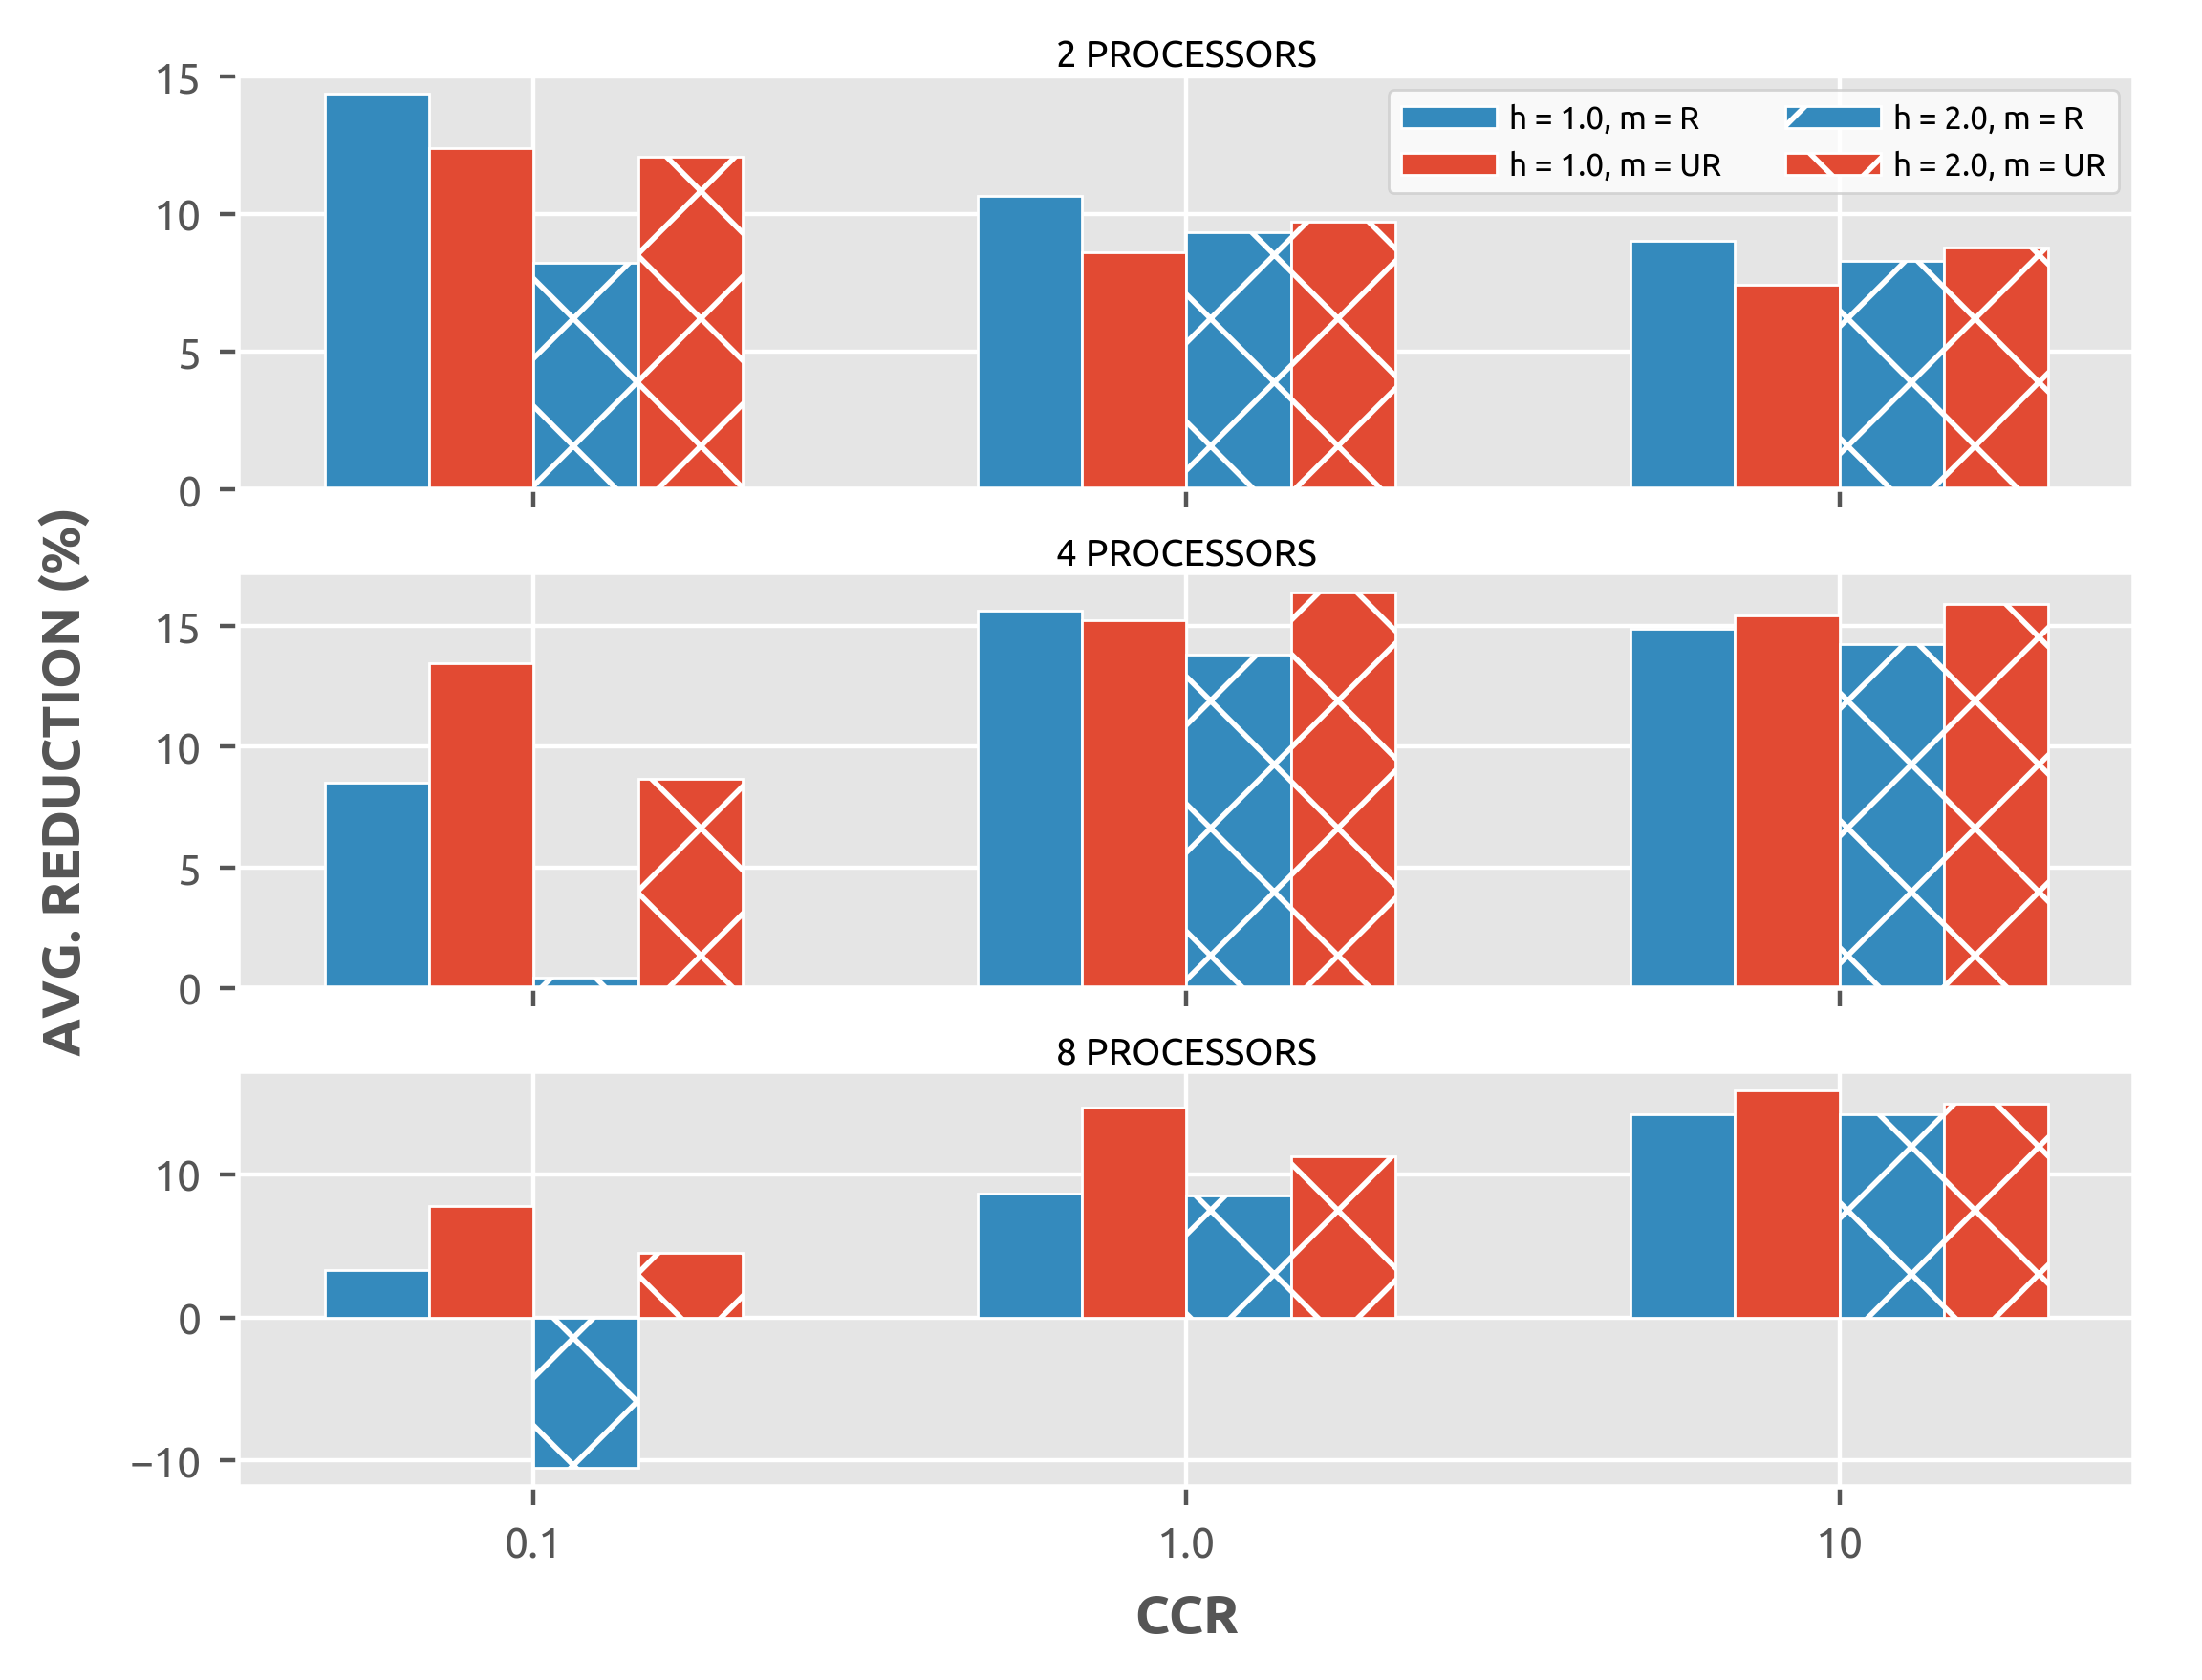
\includegraphics[scale=0.8]{100tasks_reductions.png}
	\caption{Average makespan reduction (\%) for standard HEFT ranking phase vs random topological sort.}	
	\label{plot.benchmark_reductions_100}
\end{figure}

Clearly the most interesting takeaway from the figure is the negative reduction that we see for one of the DAG sets in the bottom-left corner---i.e., the random sort did better on average for those DAGs with CCR $0.1$ and $h = 2.0$ for which costs were generated using the {\em related} method. Interestingly, the effect appears to become more pronounced as the ratio of tasks to processors decreases: the reduction is always positive for the larger DAG sets ($n = 1000$) with the same parameters, although the raw number of instances for which the random sort outperformed standard HEFT is high for those as well. 

It is not obvious why this should be so but we suspect it is related to the similar phenomenon remarked upon in the previous chapter, where HEFT failed altogether due to difficulty managing communication costs because of its greedy processor selection phase. In fact, both standard HEFT and the random ranking alternative failed altogether in the vast majority of instances for which the former was worse than the latter; the average reduction is much smaller for certain subsets because they are precisely the ones for which HEFT is most likely to struggle in general. Disregarding those instances in which both failed, the percentage of graphs for which the random sort outperformed the standard ranking was roughly $0$--$2\%$ for all subsets (of both sizes). Given this, we conclude that HEFT's task prioritization phase is clearly useful except for those circumstances when the algorithm itself struggles because of its greedy selection phase. 
% Why does HEFT do badly as #processors increases? Maybe more analysis of when HEFT does badly? Similarly, more analysis of those DAGs for which random sort did better than HEFT.  


\subsection{Evaluation of proposed rankings}
\label{subsect.evaluation}

In this section we compare the performance of HEFT when the following different number sequences are used as task priorities:
\begin{itemize}
	\item $u_i$, the standard upward ranks,
	\item $O_i$, the optimistic ranks as defined by \eqref{eq.opt_ui},
	\item $f_i$, the Fulkerson ranks as defined by \eqref{eq.f_clingen},
	\item $\hat{u}_i$, the weighted mean as defined in Section \ref{subsect.adjusting},
	\item $\hat{f}_i$, the weighted Fulkerson numbers as defined in Section \ref{subsect.adjusting}.
\end{itemize}
    

%
%Only considered Fulkerson for the smaller DAG sizes since too expensive---conclusion: doesn't appear to do any better, even the weighted version. But maybe discuss example for CPU-GPU. Monte Carlo results, same thing. 

\subsection{Conclusions}
\label{subsect.conclusions}

%Only weighted mean showed any consistent improvement...

\section{Processor selection}
\label{sect.processor_selection}


%%%%%%%%%%%%%%%%%%%%%%%%%%%%%%%%%%%%%%%%%%%%%%%%%%%%%%%%%%%%%%%%%%%%%%%%%%%%%%%%%%%%%%%%%%%%
% Bibliography.
%%%%%%%%%%%%%%%%%%%%%%%%%%%%%%%%%%%%%%%%%%%%%%%%%%%%%%%%%%%%%%%%%%%%%%%%%%%%%%%%%%%%%%%%%%%%
\bibliographystyle{myplain2-doi}
\bibliography{references,strings}

\end{document}
